\documentclass[a4paper, 12pt]{article}
\usepackage{titling}
\usepackage{array}
\usepackage{booktabs}
\usepackage{enumitem}
\usepackage{graphicx}
\usepackage{hyperref}
\usepackage{amssymb}
\usepackage{listings}
\setlength{\heavyrulewidth}{1.5pt}
\setlength{\abovetopsep}{4pt}
\setlength{\parindent}{0pt}
\graphicspath{{.}}

\usepackage[margin=1in]{geometry}

% Must be after geometry
\usepackage{fancyhdr}
\pagestyle{fancy}
\fancyhf{}
\rhead{SEE Assignment 1}
\lhead{P.Lukin, E. Ovchinnikova}
\cfoot{\thepage}

\setlength{\droptitle}{-5em}

\title{Scientific Experimentation and Evaluation  \\
				Assignment: 1.2}
\author{Petr Lukin, Evgeniya Ovchinnikova}
\date{Lecture date: $04^{th}$ October 2016}

\begin{document}



\maketitle

\section{Experiments}

Our task was to run 5 experiments each repeated at least 20 times. We ran the following experiments: forward motion for, 90$^{\circ}$ arc motion to the left, 90$^{\circ}$ arc motion to the right, 30$^{\circ}$ arc motion to the left and 30$^{\circ}$ arc motion to the right.\\
While experimenting we have realized the necessity of modifying code for 90$^{\circ}$ arc left and right motion so the robot trajectory would fit a for paper size. Moreover, to improve the process of adjustment of the robot's position on the paper. Before we had a function that makes robot to wait for a certain time before it starts moving the motors, so we could have time to adjust it to the "garage" position. Now this function is replaced with a function for waiting for a button pressing. That allows to regulate the time we need to install the robot. The modified code for forward motion for, 90$^{\circ}$ arc motion to the left, 90$^{\circ}$ arc motion to the right, 30$^{\circ}$ arc motion to the left and 30$^{\circ}$ arc motion to the right is shown below:

\begin{lstlisting}
package LegoNXT;

import lejos.nxt.LightSensor;
import lejos.nxt.Motor;
import lejos.nxt.SensorPort;
import lejos.robotics.navigation.DifferentialPilot;
import lejos.robotics.navigation.MoveController;
import lejos.util.Delay;
import lejos.nxt.Button;

public class goStraight {

	public static void main(String[] args) {
		double arcRad = 40;
		double angle = 90;
		double arcLen = Math.PI*2*arcRad*angle/360;
		double trackWidth = 12;
		Button.LEFT.waitForPressAndRelease();
		LightSensor lightSens1 = new LightSensor(SensorPort.S1);
		LightSensor lightSens2 = new LightSensor(SensorPort.S2);
		DifferentialPilot dp = new DifferentialPilot(
		MoveController.WHEEL_SIZE_NXT1, trackWidth, Motor.B,
		Motor.C, true);
		lightSens1.setHigh(100);
		lightSens2.setHigh(100);
		Button.RIGHT.waitForPressAndRelease();
		dp.setTravelSpeed(10);
		dp.travel(-arcLen);        
		dp.stop();
		Button.ESCAPE.waitForPressAndRelease();
	}
}

***

package LegoNXT;

import lejos.nxt.Motor;
import lejos.nxt.SensorPort;
import lejos.robotics.navigation.DifferentialPilot;
import lejos.robotics.navigation.MoveController;
import lejos.util.Delay;
import lejos.nxt.LightSensor;
import lejos.nxt.Button;

public class goLeft {

	public static void main(String[] args) {
		double arcRad = 25;
		double angle = 90;
		double trackWidth = 12;
		Button.LEFT.waitForPressAndRelease();
		LightSensor lightSens1 = new LightSensor(SensorPort.S1);
		LightSensor lightSens2 = new LightSensor(SensorPort.S2);
		DifferentialPilot dp = new DifferentialPilot(
		MoveController.WHEEL_SIZE_NXT1, trackWidth, Motor.B, 
		Motor.C, true);
		lightSens1.setHigh(100);
		lightSens2.setHigh(100);
		Button.RIGHT.waitForPressAndRelease();
		dp.setTravelSpeed(10);
		dp.arc(-arcRad, angle);
		dp.stop();
		Button.ESCAPE.waitForPressAndRelease();
	}
}

***

package LegoNXT;

import lejos.nxt.LightSensor;
import lejos.nxt.Motor;
import lejos.nxt.SensorPort;
import lejos.robotics.navigation.DifferentialPilot;
import lejos.robotics.navigation.MoveController;
import lejos.util.Delay;
import lejos.nxt.Button;

public class goRight {

	public static void main(String[] args) {
		double arcRad = 25;
		double angle = 90;
		double trackWidth = 12;
		Button.LEFT.waitForPressAndRelease();
		LightSensor lightSens1 = new LightSensor(SensorPort.S1);
		LightSensor lightSens2 = new LightSensor(SensorPort.S2);
		DifferentialPilot dp = new DifferentialPilot(
		MoveController.WHEEL_SIZE_NXT1, trackWidth, Motor.B, 
		Motor.C, true);
		lightSens1.setHigh(100);
		lightSens2.setHigh(100);
		Button.RIGHT.waitForPressAndRelease();
		dp.setTravelSpeed(10);
		dp.arc(arcRad, -angle);
		dp.stop();
		Button.ESCAPE.waitForPressAndRelease();
	}
}

***
package LegoNXT;

import lejos.nxt.Button;
import lejos.nxt.LightSensor;
import lejos.nxt.Motor;
import lejos.nxt.SensorPort;
import lejos.robotics.navigation.DifferentialPilot;
import lejos.robotics.navigation.MoveController;

public class goSlightlyLeft {
	public static void main(String[] args) {
		double arcRad = 120;
		double angle = 30;
		double trackWidth = 12;
		Button.LEFT.waitForPressAndRelease();
		LightSensor lightSens1 = new LightSensor(SensorPort.S1);
		LightSensor lightSens2 = new LightSensor(SensorPort.S2);
		DifferentialPilot dp = new DifferentialPilot(
		MoveController.WHEEL_SIZE_NXT1, trackWidth, Motor.B, 
		Motor.C, true);
		lightSens1.setHigh(100);
		lightSens2.setHigh(100);
		Button.RIGHT.waitForPressAndRelease();
		dp.setTravelSpeed(10);
		dp.arc(-arcRad, angle);
		dp.stop();
		Button.ESCAPE.waitForPressAndRelease();
	}
}
***
package LegoNXT;

import lejos.nxt.Motor;
import lejos.nxt.SensorPort;
import lejos.robotics.navigation.DifferentialPilot;
import lejos.robotics.navigation.MoveController;
import lejos.util.Delay;
import lejos.nxt.LightSensor;
import lejos.nxt.Button;

public class goSlightlyRight {

	public static void main(String[] args) {
		double arcRad = 120;
		double angle = 30;
		double trackWidth = 12;
		Button.LEFT.waitForPressAndRelease();
		LightSensor lightSens1 = new LightSensor(SensorPort.S1);
		LightSensor lightSens2 = new LightSensor(SensorPort.S2);
		DifferentialPilot dp = new DifferentialPilot(
		MoveController.WHEEL_SIZE_NXT1, trackWidth, Motor.B, 
		Motor.C, true);
		lightSens1.setHigh(100);
		lightSens2.setHigh(100);
		Button.RIGHT.waitForPressAndRelease();
		dp.setTravelSpeed(10);
		dp.arc(arcRad, -angle);
		dp.stop();
		Button.ESCAPE.waitForPressAndRelease();
	}
}

\end{lstlisting}	

For the experiment we used a setup described in section "4 What and how we are planning to do" of assignment 1.1with updated program code. The robot was placed on a large marked paper (Fig.\ref{fig:paper}) to a "garage" position (Fig.\ref{fig:garage}) and launched 100 times to five different directions.

\begin{figure}[h]
  \centering
  \caption{Paper with the "garage" marks.\label{fig:paper}}
  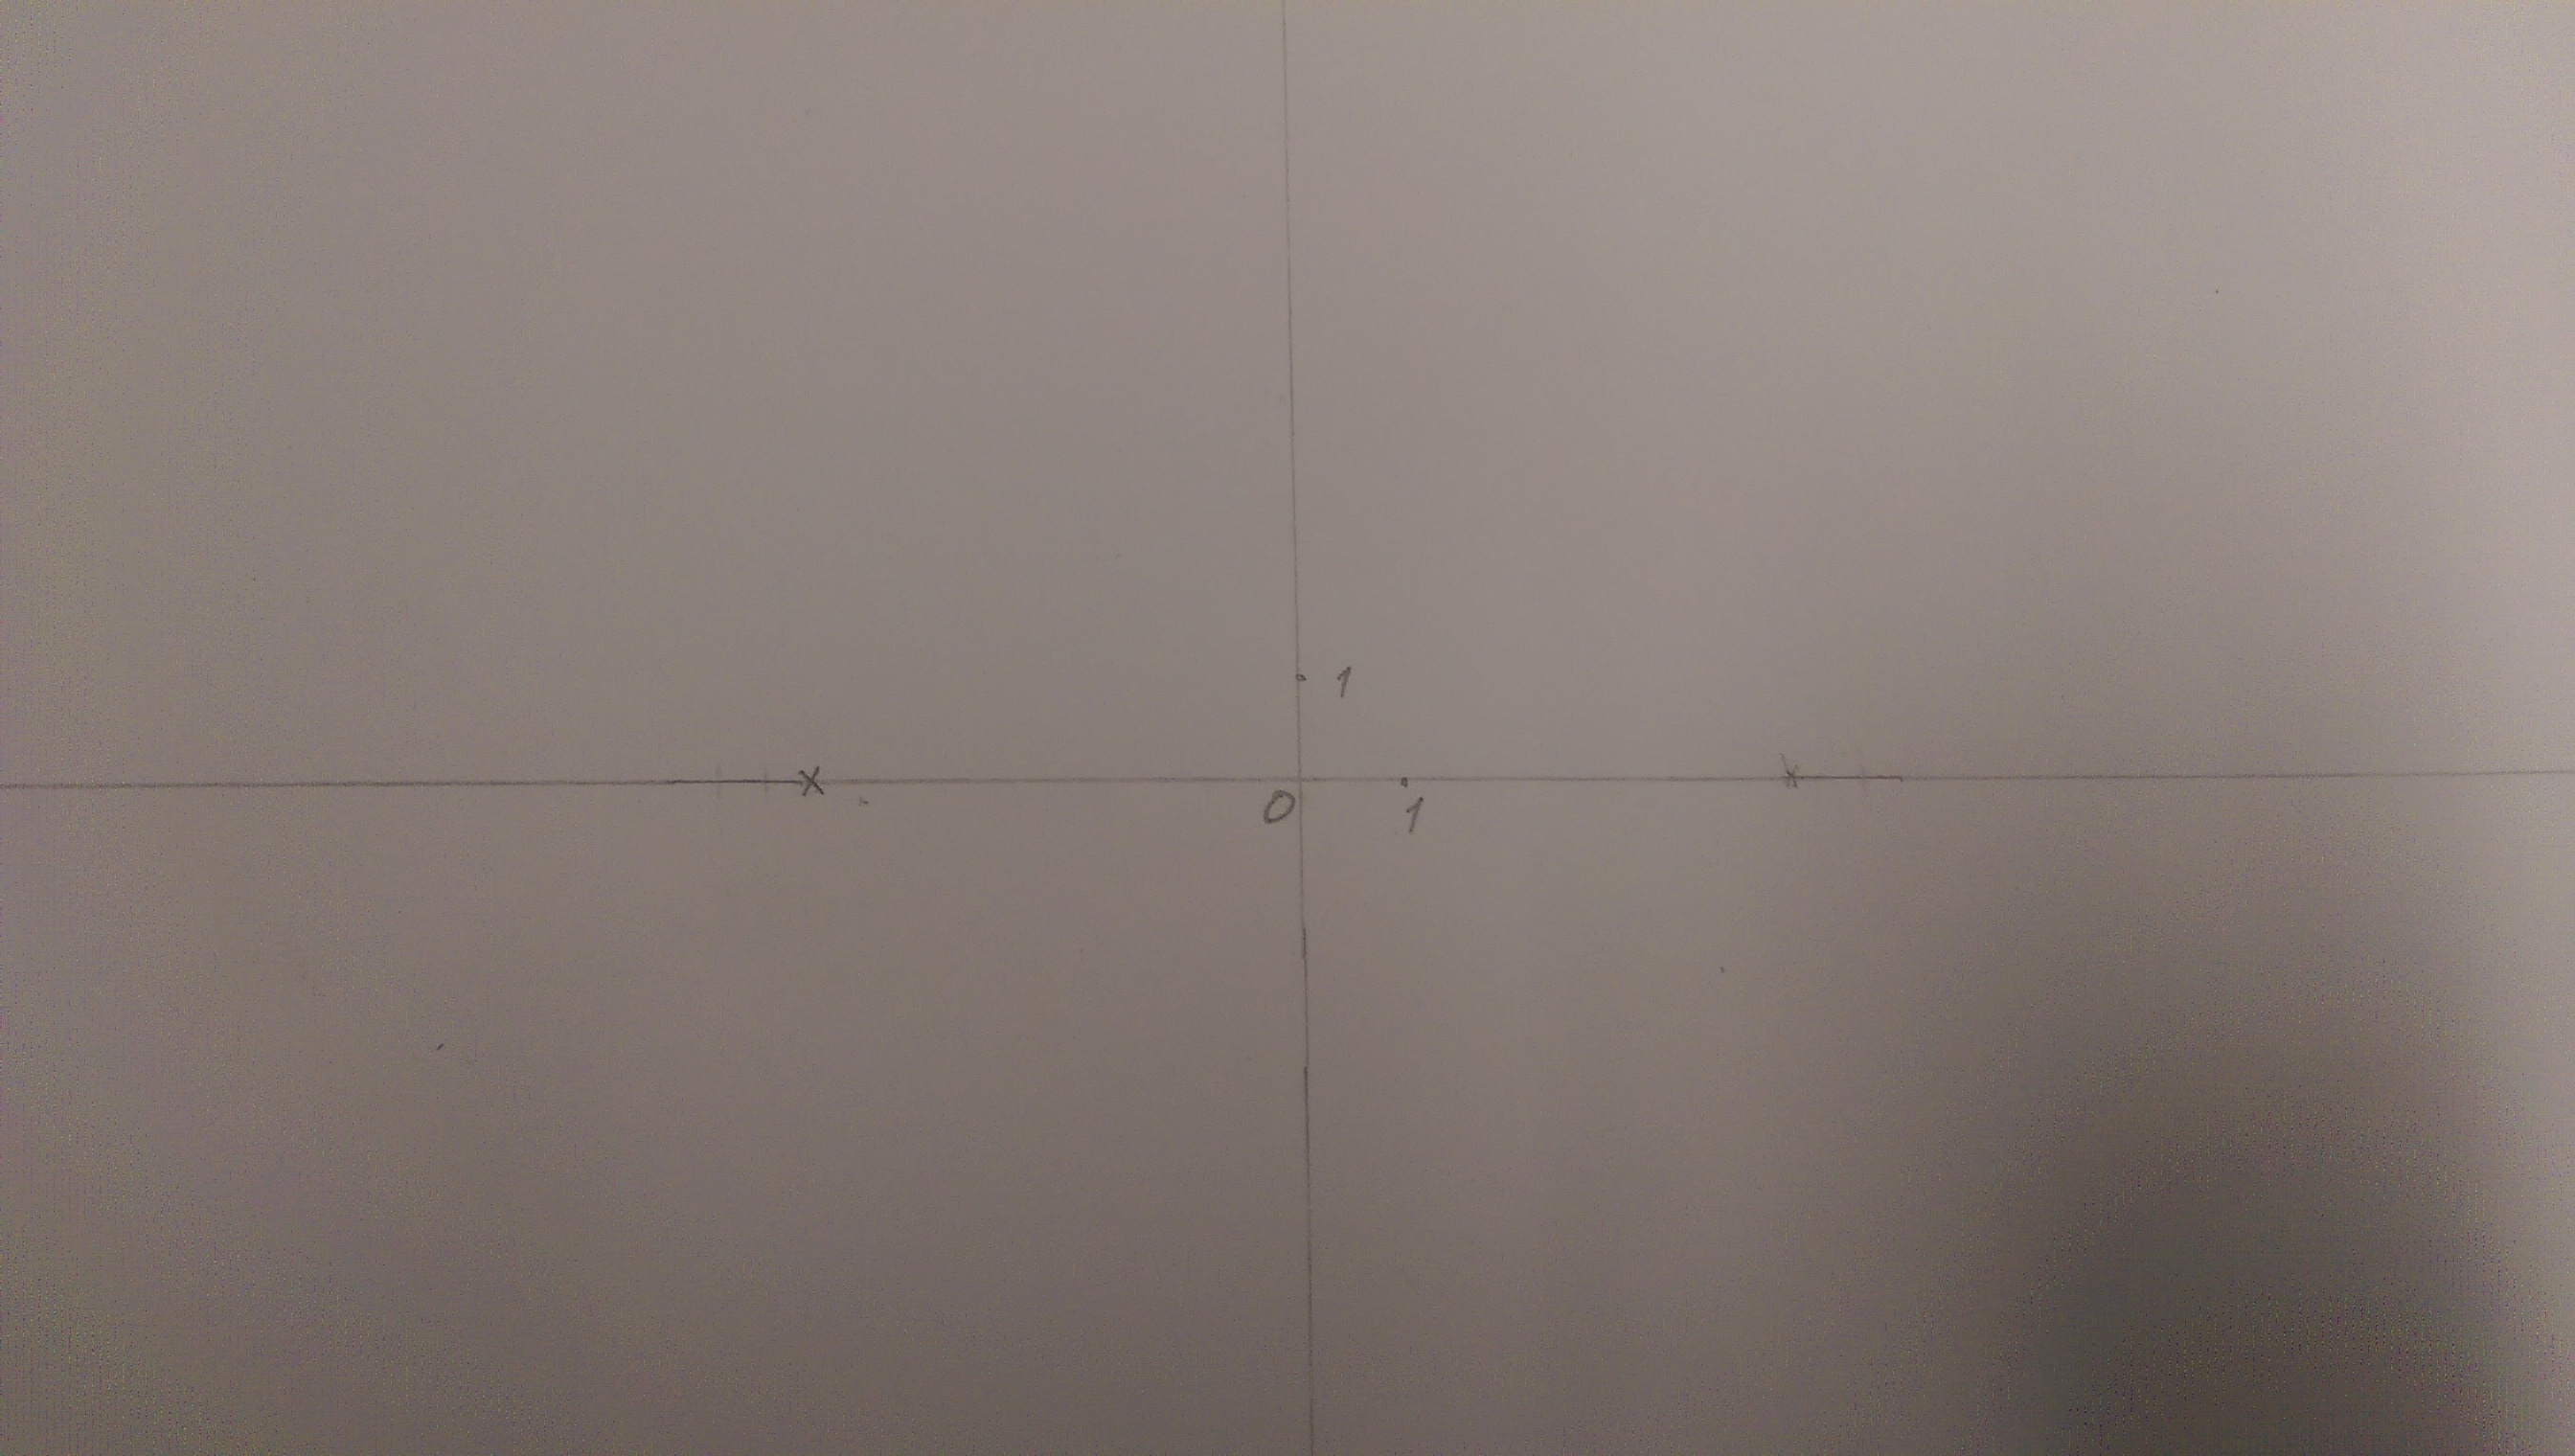
\includegraphics[width=0.8\textwidth]{markedPaper}
\end{figure}

\begin{figure}[h]
  \centering
  \caption{Robot placed into the "garage" position.\label{fig:garage}}
  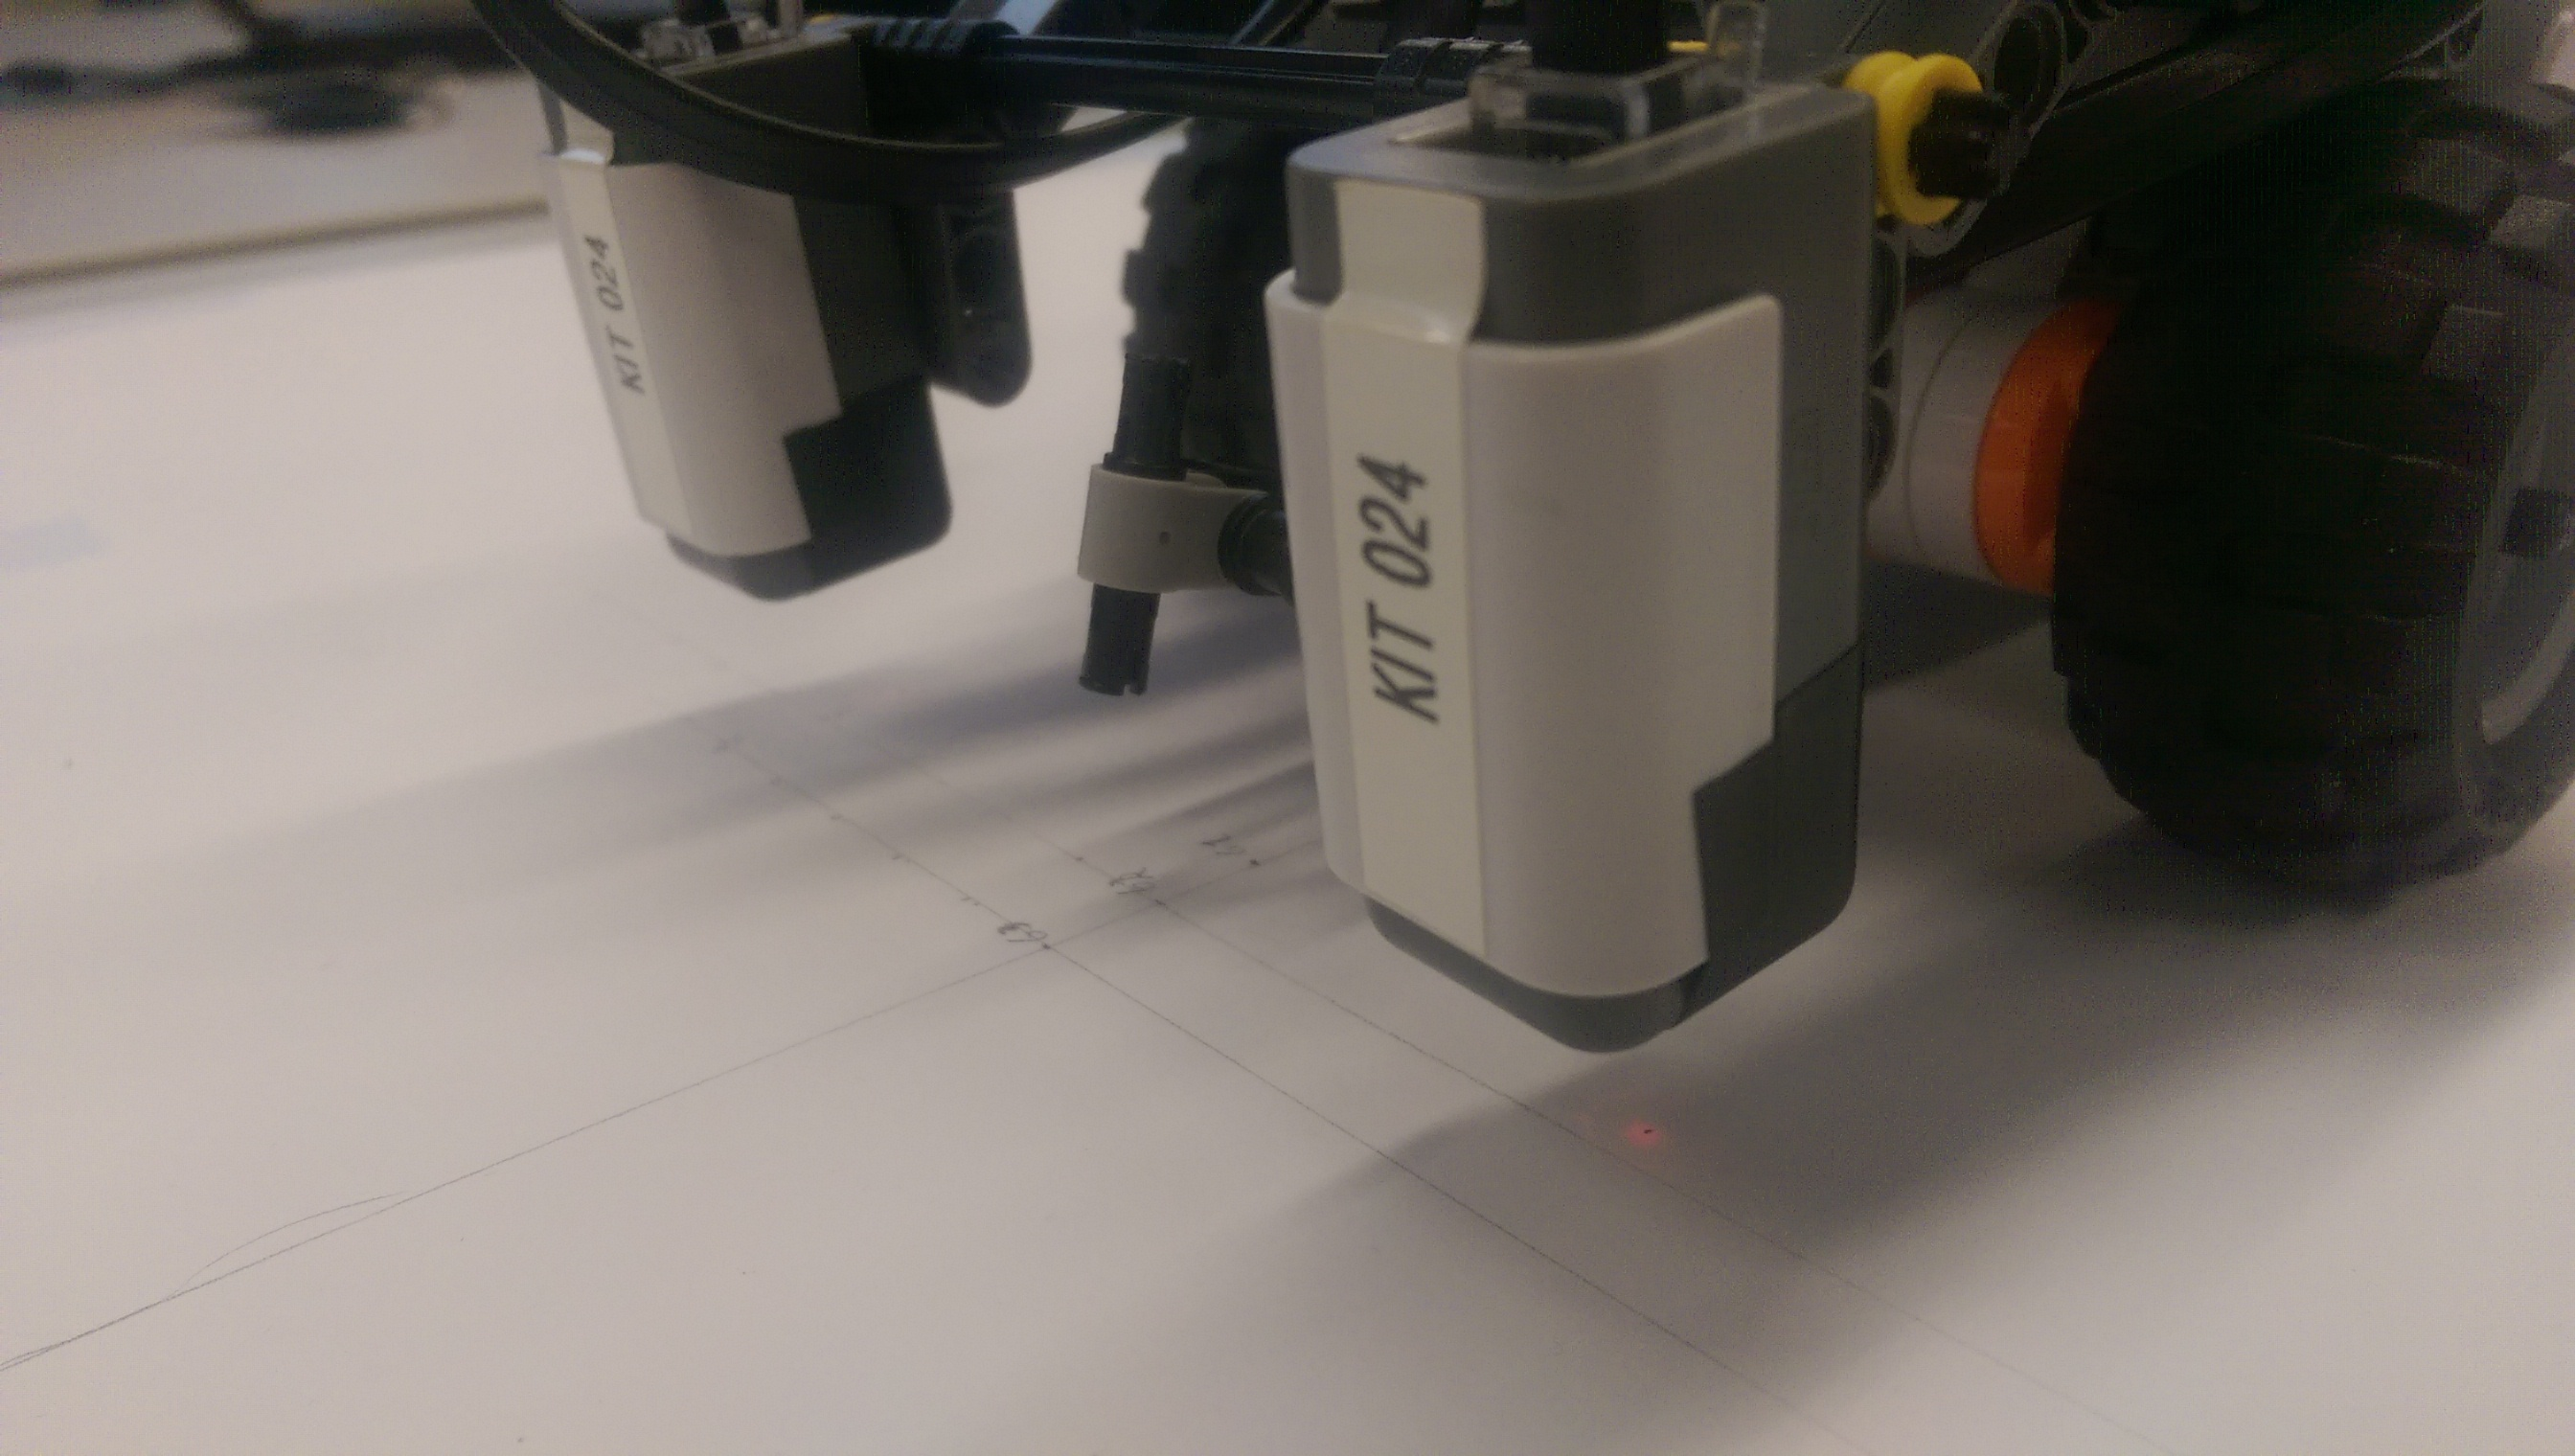
\includegraphics[width=0.8\textwidth]{garage}
\end{figure}




\section{Experimental results processing}

\section{Conclusions}
During the experiment we have noticed two new possible error sources. First, we have a flexible caster wheel (Fig), that is impossible to put in the perfectly same position each time we redo the experiment. 

//TODO: insert the wheel image

That is an unavoidable error, that can be eliminated only by using a completely different construction of the robot. Second, though the button pressing control is convenient and allow us to install the robot without time limits, the act of pressing can slightly move the robot. However, after several tests on short distances, where the motor error is still not too big, we've concluded that this error is insignificant and cannot be detected by our measurement methods.

\end{document}
